\documentclass[11pt]{kasper}
% 
% If you do not have 'kasper.cls', see
% http://www.damtp.cam.ac.uk/user/kp229/texstuff .

\usepackage{makeidx}
\usepackage{verbatim}
\usepackage{relsize}
\makeindex
%\newcommand{\toindex}[1]{#1\index{#1}}

\newcommand{\member}[1]{{\tt #1}\index{#1}}
%\newcommand{\member}[1]{{\tt #1}}

\def\mystrut{\vbox to 8.5pt{}\vtop to 3.5pt{}}
\def\V{\hskip10pt\vrule\hskip10pt}
\def\T{\hskip10pt\vrule\vrule height2.5pt depth -2.1pt width 10pt}
\def\L{\hskip10pt\vrule height 8.5pt depth -2.1pt
       \vrule height2.5pt depth -2.1pt width 10pt}
\def\N{\hskip10pt\phantom{\vrule}\hskip10pt}
\def\hw{\hskip-1000pt plus 1fil}

% to test: insert before end of subtree

\begin{document}
\title{{\tt tree.hh} documentation}
\author{Kasper Peeters}
\email{kasper.peeters@gmail.com}
\maketitle
\begin{abstract}
The {\tt tree.hh} library for C++ provides an STL-like container class
for n-ary trees, templated over the data stored at the nodes.  Various
types of iterators are provided (post-order, pre-order, and
others). Where possible the access methods are compatible with the STL
or alternative algorithms are available. The library is available
under the terms of the GNU General Public License.\\[3ex]
Code and examples available at: {\tt http://tree.phi-sci.com/}\\[3ex]
{\bf This documentation is not yet entirely complete. Refer to the {\tt
tree.hh} header file for a full list of member functions.}
\end{abstract}
\vfill
\maketoc
\eject

\begin{sectionunit}
\title{Overview}
\maketitle
\begin{sectionunit}
\title{The container class}
\maketitle
The tree class of {\tt tree.hh} is a templated container class in the
spirit of the STL. It organises data in the form of a so-called n-ary
tree. This is a tree in which every node is connected to an arbitrary
number of child nodes. Nodes at the same level of the tree are called
``siblings'', while nodes that are below a given node are called its
``children''. At the top of the tree, there is a set of nodes which
are characterised by the fact that they do not have any parents. The
collection of these nodes is called the ``head'' of the tree. See
figure~\ref{f:overview} for a pictorial illustration of this
structure (90 degrees rotated for convenience).
\begin{figure}[th]
\begin{center}
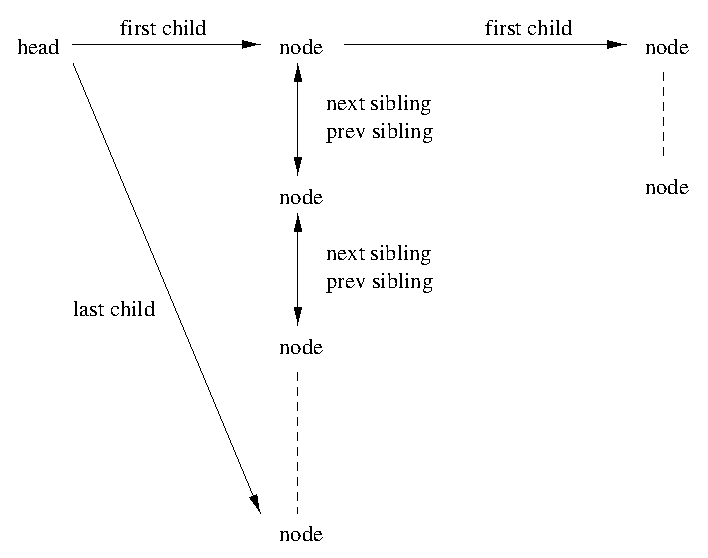
\includegraphics[width=.5\textwidth]{treefig}
\caption{Overview of the tree structure. The elements at the top of
the tree (here displayed at the left for convenience) are in the
``head'' (there can be more than one such element).  Every node is
linked to its children using the ``first child'' and ``last child''
links. In addition, all nodes on a given level are doubly-linked using
the ``previous sibling'' and ``next sibling'' links. The ``depth'' of
a given node refers to the horizontal distance from the head nodes.}
\label{f:overview}
\end{center}
\end{figure}

The tree class is templated over the data objects stored at the nodes;
just like you can have a {\tt vector<string>} you can now have a
{\tt tree<string>}. Many STL algorithms work on this data structure,
and where necessary alternatives have been provided.
\medskip

\end{sectionunit}
\begin{sectionunit}
\title{Iterators}
\maketitle

The essential difference between a container with the structure of a
tree and the STL containers is that the latter are ``linear''. While
the STL containers thus only have essentially one way in which one can
iterate over their elements, this is not true for trees. The {\tt
tree.hh} library provides (at present) four different iteration
schemes. To describe them, consider the following tree:
\begin{equation*}
\vcenter{\offinterlineskip
\halign{&#\mystrut\hfil\cr
 root \hw\cr
 \T A \cr
 \V   \T  B \cr
 \V   \L  C \cr
 \L D \cr
 \N   \T  E \cr
 \N   \L  F \cr}}
\end{equation*}
The three iteration types and the resulting order in which nodes are
visited are tabulated below:
\begin{center}
\begin{tabular}{llll}
pre-order (default) & ``element before children'' &
\member{pre\_order\_iterator}  & root A B C D E F \\
post-order          & ``element after children''  &
\member{post\_order\_iterator} & B C A E F D root \\
breadth-first &  &
\member{breadth\_first\_iterator} & root A D B C E F  \\
sibling             & ``only siblings'' & 
\member{sibling\_iterator} & (for ex.) A D \\
fixed-depth         & &
\member{fixed\_depth\_iterator} & (for ex.) A D \\
leaf                & &
\member{leaf\_iterator} & B C E F
\end{tabular}
\end{center}
The pre-order ones are the default iterators, and therefore also known
under the name of {\tt iterator}. Sibling iterators and fixed-depth
iterators iterate only over the nodes at a given depth of the
tree. The former restrict themselves to the child nodes of one given
node, while the latter iterates over all child nodes at the given
depth. Finally, leaf iterators iterate over all leafs (bottom-most)
nodes of the tree.

There are copy constructors that will convert iterators of the
various types into each other. The post- and pre-order iterators are
both also known as ``depth-first'', in contrast to the
``breadth-first'' iterator.

The begin and end iterators of a tree can be obtained using
\member{begin()} and \member{end()} (for pre-order iterators) or
alternatively \member{begin\_post()} and \member{end\_post()} (for
post-order iterators) and \member{begin\_leaf()} and
\member{end\_leaf()} (for leaf iterators). Similarly, the begin and
end sibling iterators can be obtained by calling
\member{begin(iterator)} and \member{end(iterator)}.  The range of
children of a given node can also be obtained directly from an
iterator, by using the {\tt iterator::begin()} and {\tt
iterator::end()} member functions.

If you want to (temporarily) make an iterator not go into the child
subtree, call the member function \member{skip\_children}. This will only
keep effect for a single increment or decrement of the
iterator. Finally, whether or not an iterator is actually pointing at
a node (i.e.~is not an ``end'' iterator) can be tested using the
\member{is\_valid(iterator)} member of the tree class.

\end{sectionunit}
\end{sectionunit}

\begin{sectionunit}
\title{Basic operations}
\maketitle
\begin{description}
\item[Initialising] There are two nontrivial constructors. One which takes 
a single node element as argument. It constructs a tree with this node
begin the sole node in the head (in other words, it is a combination
of a trivial constructor together with a \member{set\_head} call).
The other non-trivial constructor takes an iterator, and copies the
subtree starting at that node into the newly created tree (useful for
constructing new tree objects given by subtrees of existing trees).

\item[Tree traversal] Besides the \member{operator++} and
\member{operator--} members for step-wise traversal through the tree,
it is also possible to use the \member{operator+=} and \member{operator-=}
member functions to make more than one step at the same time (though
these are linear time, not amortized constant). The result of stepping
beyond the end of the tree or stepping beyond the end of a sibling
range (for sibling iterators) is undefined.

The parent of a given node can be reached by calling the \member{parent}
member of the tree object, giving it an iterator pointing to the node.

If you know the number of children of a given node, you can get direct
access to the $n$th child by using the \member{child} member
function. Note that the value of the index is not checked and should
therefore always be valid.

\item[Appending child nodes] Nodes can be added as children of a given
node using the \member{append\_child} member function.

\item[Inserting nodes] Nodes can be inserted at the same depth as a
given other node using the \member{insert} and \member{insert\_after}
members functions. This is also how you insert the first node into a 
tree.
\end{description}
\end{sectionunit}

\begin{sectionunit}
\title{Other algorithms}
\maketitle
\begin{sectionunit}
\title{Non-mutating algorithms}
\maketitle
\begin{description}
\item[Counting nodes] The total number of nodes of a tree can be
obtained using the \member{size} member function, while the number of
children of a given node can be obtained with a call to
\member{number\_of\_children(iterator)}. Similarly, the number of
nodes at a given depth (the number of siblings of a given node) can be
obtained using the \member{number\_of\_siblings} member function.
\item[Determining depth] The \member{depth()} member function returns the
distance of a node to the root.
\item[Accessing siblings by their index] See the next item.
\item[Determining index in a sibling range] In order to determine the
index of a node in the range of siblings to which it belongs, use the
\member{index(sibling\_iterator)} member function. The first sibling node
has index 0. The reverse of this function (obtaining a sibling node
given its index in the range of siblings) is called
\member{child(const iterator\_base\&, unsigned int)}.
\item[Comparing trees] While the STL \member{equal} algorithm can be used 
to compare the values of the nodes in two different trees, it does not 
know about the structure of the tree. If you want the comparison to
take this into account, use the \member{equal(iterator, iterator,
iterator, BinaryPredicate)} call of the tree class. As an addition to
the STL algorithm, the length of the first range does not have to be
equal to the length of the range pointed to by the second iterator.

There is also an \member{equal\_subtree} algorithm which takes only
two iterators, pointing to the (single-node) heads of two
subtrees.
\end{description}
\end{sectionunit}

\begin{sectionunit}
\title{Mutating algorithms}
\maketitle
\begin{description}
\item[Erasing nodes and subtrees] In order to remove a node including
its children from the tree, use the \member{erase(iterator)} call. If you
just want to erase the children, but not the node itself, use the 
\member{erase\_children(iterator)} call. 

Erasing all siblings to the left or right of a given node is done
using \member{erase\_left\_siblings(iterator)} and
\member{erase\_right\_siblings(iterator)} respectively.

\item[Replacing individual nodes or subtrees] 

\item[Flattening subtrees] The procedure of moving all children of a
given node to be siblings of that node is called ``flattening''; it
acts as
\begin{equation*}
\vcenter{\offinterlineskip
\halign{&#\mystrut\hfil\cr
 apple \hw\cr
 \T banana\cr
 \V   \T  pear \cr
 \V   \T  strawberry \cr
 \V   \L  cherry \cr
 \L grape\cr}}\quad\rightarrow\quad
\vcenter{\offinterlineskip
\halign{&#\mystrut\hfil\cr
 apple \hw\cr
 \T banana\cr
 \T  pear \cr
 \T  strawberry \cr
 \T  cherry \cr
 \L grape\cr}}
\end{equation*}
% \begin{screen}
% apple                       apple
% 	  banana                      banana
% 		  pear            ->       pear
% 		  strawberry               strawberry
% 		  cherry                   cherry
% 	  grape                       grape
% \end{screen}
when the tree is flattened at the ``banana'' node.

\item[Moving or exchanging subtrees] Simple exchange of one sibling node with the
next one is done through the member function \member{swap(sibling\_iterator)}. The
iterator remains valid and remains pointing to the moved subtree.

More complicated move operations are the \member{move\_ontop},
\member{move\_before} and \member{move\_after} ones. These all take
two iterators, a source and a target. The member
\member{move\_ontop(target, source)} removes the `target' node and
all its children, and replaces it with the `source' node and its
children.  The `source' subtree is removed from its original location.
The other two move members do a similar thing, differing only in the
node which is to be replaced.

\item[Extracting subtrees] You can create a new tree object
filled with the data of a subtree of the original tree. This is
analogous to the extraction of a substring of a string. The relevant
member function is \member{subtree(sibling\_iterator,
sibling\_iterator)} which takes a range of siblings as argument. 
There is also a slight variation of this member, which does not return
a tree object but instead populates one that is passed as an argument
(useful if you want to call this on a tree object subclassed from
{\tt tree<T>}.

\item[Sorting] The standard STL sort algorithm is not very useful for
trees, because it only exchanges values, not nodes. Applying it to a
tree would mean that the structure of the tree remains unmodified,
only node values get moved around (not their subtrees).

Therefore, the {\tt tree} class has its own sort member. It comes in
two forms, just like the STL sort, namely
\begin{screen}
void     sort(sibling_iterator from, sibling_iterator to, bool deep=false);

template<class StrictWeakOrdering>
void     sort(sibling_iterator from, sibling_iterator to,
              StrictWeakOrdering comp, bool deep=false);
\end{screen}
The result of a call to either of these is that the nodes in the range
described by the two iterators get sorted. If the boolean {\tt deep}
is true, the subtrees of all these nodes will get sorted as well (and
so one can sort the entire tree in one call).  As in the STL, you can
use the second form of this function to pass your own comparison
class.

If the nodes to which the two iterators point are not in the same
sibling range (i.e.~not at the same depth in the tree), the result is undefined.

\item[Merging] One way in which one might think of indicating the
position where new nodes are to be inserted, is to give the path that
leads to the insertion point.  For instance, given the tree
\begin{equation*}
\vcenter{\offinterlineskip
\halign{&#\mystrut\hfil\cr
 apple \hw\cr
 \T banana\cr
 \V   \T  pear \cr
 \V   \T  strawberry \cr
 \V   \L  cherry \cr
 \L grape\cr}}
\end{equation*}
one could imagine using the sub-tree
\begin{equation*}
\vcenter{\offinterlineskip
\halign{&#\mystrut\hfil\cr
 apple \hw\cr
 \L banana\cr
 \N   \T  coconut \cr
 \N   \L  raspberry \cr}}
\end{equation*}
to indicate that the nodes ``coconut'' and ``raspberry'' are to be
inserted as new children of the ``banana'' node. In {\tt tree.hh} this
process is called \emph{tree merging}. It can do the simple addition
of children as above, but actually handles the generic case too: as
an example consider the merge
\begin{equation*}
\text{\tt merge}\left[
\vcenter{\offinterlineskip
\halign{&#\mystrut\hfil\cr
 apple \hw\cr
 \T banana\cr
 \V   \T  pear \cr
 \V   \T  strawberry \cr
 \V   \L  cherry \cr
 \T grape\cr
 blueberry \cr}}\quad, \quad
\vcenter{\offinterlineskip
\halign{&#\mystrut\hfil\cr
 apple \hw\cr
 \T banana\cr
 \V   \T coconut \cr
 \V   \L raspberry \cr
 \T tangerine \cr
 \V   \L plum\cr
 blueberry \cr
 \N   \L orange \cr}}\right]\quad\rightarrow\quad
\vcenter{\offinterlineskip
\halign{&#\mystrut\hfil\cr
 apple \hw\cr
 \T banana\cr
 \V   \T pear\cr
 \V   \T strawberry\cr
 \V   \T cherry\cr
 \V   \T coconut \cr
 \V   \L raspberry \cr
 \T grape\cr
 \T tangerine \cr
 \V   \L plum\cr
 blueberry \cr
 \N  \L orange \cr}}
\end{equation*}
As is clear from the above, the arguments to \member{merge} are two
sibling ranges.
\end{description}
\end{sectionunit}
\end{sectionunit}

\printindex
\end{document}
